%86
\begin{frame}
  Vastag kliens alkalmazásokhoz hasonlóan adatok gyűjthetőek űrlapokkal, amiket 
  \begin{itemize}
    \item feldolgoztathatunk a szerver oldalon (most ez lesz), vagy
    \item JavaScript programmal a kliensen.
  \end{itemize}
  Űrlap vezérlők a \texttt{<form>} elembe ágyazva használhatók. Legfontosabb attribútumai:
  \begin{description}[m]
    \item[\texttt{action}] \hfill \\ A szerver oldali feldolgozó script URL-je
    \item[\texttt{target}] \hfill \\ Hova töltse a szerver válaszát 
    (\texttt{\_blank}, \texttt{\_self} (alapért.), \texttt{\_parent}, \dots)
    \item[\texttt{novalidate}] \hfill \\ Ne végezzen input 
    ellenőrzést a böngésző
    \item[\texttt{autocomplete}] \hfill \\ Korábban megadottak alapján 
    kiegészíti az adatokat (\texttt{on} (alapért.), \texttt{off})
  \end{description}
\end{frame}

%87
\begin{frame}
  \begin{description}[m]
    \item[\texttt{method}] \hfill \\ Adattovábbítási módszer:
    \begin{description}[m]
      \item[\texttt{get}] \hfill \\ Alapértelmezett. URL lekérdező 
      karakterláncában továbbítja az adatokat.
      \begin{itemize}
        \item Az URL betehető a könyvjelzők közé, és
        \item a böngészőben is könnyen szerkeszthető
      \end{itemize}
      \item[\texttt{post}] \hfill \\ HTTP tranzakcióként továbbít.
      \begin{itemize}
        \item Nincsenek méretkorlátok (URL hossza korlátozott, 
        $\approx$ 2000 karakter)
        \item Fájlok csak így továbbíthatók
        \item A böngészőben nem látszik, de ettől még \kiemel{nyílt 
        szöveg}ként továbbítják a hálózaton!
      \end{itemize}
    \end{description}
  \end{description}
\end{frame}

%88
\begin{frame}
  \begin{description}[m]
    \item[\texttt{enctype}] (type of encoding) \hfill \\ Meghatározza 
    a küldött adatok kódolását. Kötelező megadni, ha a \texttt{method} 
    attr. értéke \texttt{post}. Lehetséges értékek:
    \begin{description}[m]
      \item[\texttt{application/x-www-form-urlencoded}] \hfill \\ 
      Alapértelmezett. Minden szóközt és speciális karaktert 
      helyettesít.
      \item[\texttt{multipart/form-data}] \hfill \\ Fájlok küldésekor 
      kell használni.
      \item[\texttt{\texttt{text/plain}}] \hfill \\ Csak a szóközöket 
      helyettesíti.
    \end{description}
  \end{description}
\end{frame}

%89
\begin{frame}
  A legtöbb vezérlő az \texttt{<input>} elemmel hozható létre, pl. 
  egy számbeviteli mező néhány attribútuma, és hatása:
  \begin{description}[m]
    \footnotesize
    \item[\texttt{type}] \hfill \\ \texttt{number}, számbeviteli mező 
    létrehozása
    \item[\texttt{name}] \hfill \\ A szerver oldalon ez lesz az adat 
    \emph{kulcsa}
    \item[\texttt{min}] \hfill \\ A legkisebb bevihető érték
    \item[\texttt{max}] \hfill \\ A legnagyobb bevihető érték
    \item[\texttt{step}] \hfill \\ Ennyit változtatnak a 
    léptetőgombok/kurzurvezérlő nyilak az értéken, ennyi 
    többszöröseit lehet megadni, illetve ha 
    értéke \texttt{any}, akkor bármilyen racionális szám megadható
    \item[\texttt{required}] \hfill \\ A mező kitöltése kötelező
  \end{description}
\end{frame}

%90
\begin{frame}
  Űrlapbeküldő gomb: \texttt{<input>} elem
  \begin{itemize}
    \item \texttt{type="submit"}
    \item \texttt{value} attr. adja meg a gomb feliratát
  \end{itemize}
  \vfill
  Cimke létrehozása vezérlőhöz: \texttt{<label>} elemmel. A 
  cimkére kattintva a vezérlő is aktiválódik (pl. rádiógombnál 
  kiválasztás). Kapcsolat cimke és 
  vezérlő között:
  \begin{itemize}
    \item vezérlő a cimke belsejébe ágyazva
    \item a cimke \texttt{for} attribútumában megadható a vezérlő 
    \texttt{id}-je
  \end{itemize}
\end{frame}

%91
\begin{frame}
  Vezérlők logikai csoportosítása: \texttt{<fieldset>} elemmel\\
  Csoport feliratának megadása: \texttt{<legend>} elemben
  \vfill
  \begin{center}
    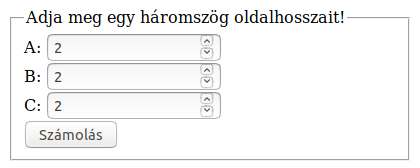
\includegraphics[width=.5\textwidth]{urlap1.png}
  \end{center}
\end{frame}

%92
\begin{frame}
  \begin{exampleblock}{\textattachfile{urlap1.html}{urlap1.html} 
  (\textattachfile{urlap1.php}{urlap1.php})}
    \footnotesize
    \lstinputlisting[style=HTML,linerange={8-20},numbers=left,firstnumber=8]{urlap1.html}
  \end{exampleblock}
\end{frame}

%93
\begin{frame}
  A legtöbb vezérlő az \texttt{<input>} elemmel és annak \texttt{type} 
  attribútumával állítható elő. Az összes vezérlővel használható főbb 
  attribútumai: 
  \begin{description}[m]
    \item[\texttt{autocomplete}] \hfill \\ Automatikus kiegészítés a 
    korábban begépelt tartalom alapján. (\texttt{on}, \texttt{off}) 
    \item[\texttt{autofocus}] \hfill \\ Oldalbetöltés után 
    automatikusan fókuszba kerül 
    \item[\texttt{disabled}] \hfill \\ Letiltott vezérlő 
    \item[\texttt{form}] \hfill \\ Ha a vezérlő 
    nincs \texttt{<form>} elembe ágyazva, akkor annak \texttt{id}-je 
    alapján logikailag összekapcsolható vele.
  \end{description}
\end{frame}

%94
\begin{frame}
  \begin{description}[m]
    \item[\texttt{id}] \hfill \\ A vezérlőt egyedileg azonosítja a 
    \kiemel{kliens} oldalon (pl. JavaScript programokban)
    \item[\texttt{name}] \hfill \\ A vezérlőt azonosítja a 
    \kiemel{szerver} oldalon (kulcs) 
    \item[\texttt{readonly}] \hfill \\ Csak olvashatóvá teszi a vezérlőt 
    \item[\texttt{required}] \hfill \\ A mező kitöltése kötelező 
    \item[\texttt{value}] \hfill \\ A vezérlő értéke
  \end{description}
\end{frame}

%95
\begin{frame}
  Egysoros szövegbeviteli mező: \texttt{type="text"} (alapértelmezés)
  \begin{description}[m]
    \item[\texttt{list}] \hfill \\ Egy \texttt{<datalist>} elem (ajánlatok legördülő listája) \texttt{id}-jét tartalmazza
    \item[\texttt{maxlength}] \hfill \\ A begépelhető karakterek száma
    \item[\texttt{pattern}] \hfill \\ Reguláris kifejezés az érték ellenőrzéséhez
    \item[\texttt{placeholder}] \hfill \\ Helyőrző, ami az első karakter begépeléséig segít a felhasználónak, pl. ,,A rendszámot kötőjel nélkül, nagybetűkkel adja meg!''
    \item[\texttt{size}] \hfill \\ A vezérlő szélessége átlagos karakterszélességben mérve (CSS jobb)
  \end{description}
\end{frame}

%96
\begin{frame}
  A \texttt{<datalist>} elembe \texttt{<option>} elemek ágyazhatók, 
  melyek gépelést segítő legördülő lista elemeiként jelennek meg.\\
  A (\texttt{<select>} elemben is használható) \texttt{<option>} attribútumai:
  \begin{description}[m]
    \item[\emph{attribútum nélkül}] \hfill \\ Az elem tartalma jelenik meg a legördülő listában, és ezt továbbítják a szervernek is
    \item[\texttt{label}] \hfill \\ A listában egy rövidebb szöveg jelenhet meg, mint az elem értéke
    \item[\texttt{selected}] \hfill \\ Kiválasztottá teszi az elemet az oldal betöltésekor
    \item[\texttt{value}] \hfill \\ Ha megadják, ennek tartalmát küldi a szervernek, nem a megjelenő szöveget
  \end{description}
\end{frame}

% reguláris kifejezések ismertetése!
